\chapter{Einleitung}
\label{sec:einleitung} 

Die Computer Vision gehört zum Fachbereich der Computer Science und beinhaltet vor allem die Entwicklung von künstlichen Intelligenzen, allen voran dem Versuch Computern ein visuelles Verständnis ihrer Umgebung zu geben. Das Ziel der Computer Vision ist es das menschliche Auge zu simulieren. Das menschliche Verständnis über die sich ihm umgebenden Welt, ist auf seine Fähigkeit Entscheidungen auf Grund visueller Eindrücke und deren Interpretation, zurückzuführen. Computer, welche die Fähigkeit besitzen die Welt um sich herum wie das menschliche Auge zu betrachtet und aus diesen entstehenden Bildern Informationen zu extrahieren, wären dem zu folge auch in der Lage Entscheidungen auf Grund von visuellen Eindrücken zu fällen und entsprechend zu handeln. Die Simulation erfordert insgesamt drei Schritte. Als erstes muss die anloge Umgebung in digitale für der Computer verständliche Bilder umgewandelt werden. Die erfolgt mit Hilfe von Kameras, Sensoren oder Lasern, welche die Umgebung als digitale Bilder an den Computer weitergeben. Im zweiten Schritt erfolgt die Bildverarbeitung. mit Hilfe von Detektionsalgorithmen werden markante Punkte auf den aufgenommen Bilder herausgefiltert, dazu gehören beispielsweise die Kanten und Ecken-Erkennung, die Segmentierung von Bildern in einzelne sich nicht überlappende Teilbereiche und anschließene Klassifizierung sowie Merkmals Erkennungen. Der dritte Schritt ist dann eine zusammenführung der ersten beide Schritte. Jetzt werden aus den Bilddaten und den Merkmalen, welche durch den Bildverabeitung entstanden sind, informationen über die Umgebung berechnet. Dazu gehören unter anderem das rekonstruieren des 3D-Raumes oder die Objekterkennung von Objekte im Raum, sowie auch deren Bewegungsverfolgung, falls diese nicht statisch sind. Beispiele für auf Computer Vision basierende Applikationen sind im Bereich des Autonomen Fahrens, Motion-Capturing-Anlagen, Bewegungserkennungen oder Service Robotern zu finden. Mit dem Entwickeln von Algorithmen für Computer Vision Applikationen, sieht man sich mit immer wieder mit komplizierten Aufgaben und Herausforderungen konfrontiert. Bei der Aufnahme von Bildern, kann es immer wieder zu unvorhersehbaren Bildfehlern wie beispielsweise Rauschen oder Verzerrungen durch die Kameralinse kommen, was auch nicht oft zum Verlust von Referenzdaten führt. Des Weiteren muss mit limitierten Ressourcen wie Speicher oder Rechenleistung geschickt umgegangen werden, gerade im Bereich der Echt-Zeit-Verarbeitungen von Daten, wie sie im Motion-Capturing oder im autonomen Fahren verlangt werden. Computer Vision kommt immer dann zum Einsatz, sobald Informationen aus Bildern gewonnen werden sollen. Dabei kann man unterscheiden unter der Informationsgewinnung aus einzel Bildern oder bewegt Bildern, genauso wie single-view, two-view oder multiple-view Aufnahmen. Single-View beschreibt die Bildverarbeitung anhand der Aufnahmen einer Kamera, two-view befasst sich mit Stereoskopischen Aufnahmen und involviert zwei Kameras und multiple-view ist die Zusammenfassung von mehr als zwei Kameras, wie sie beispielsweise im Motion-Capturing verwendet werden. Um eine dreidimensionale Interpretation von Objekten und deren Orientierung im Raum, basierend auf Bilddaten von Kameras, zu bekommen, muss in irgendeiner Form bestimmte Parameter des verwendeten Kameramodells bekannt sein oder herausgefiltert werden. Dieser Vorgang wird als Kamerakalibrierung bezeichnet und beschreibt die Gewinnung von extrinsischen und intrinsischen Kameraparametern\cite{HZ,Ferid,Elements,ZZGXr}. Als extrinsische oder auch äußeren Kameraparameter wir die Orientierung der Kamera im Raum beschrieben, diese wird in einer 3X4-Matrix ausgedrückt, welche sowohl die Rotation der Kamera also auch deren Translation umfässt. Die intrinsischen Kameraparameter oder auch inneren Kameraparameter werden in der sogenannten Kameramatrix zusammengefasst, welche je nach benutzten Kameramodell sich unterscheidet. Die extrinsischen  und intrinsischen Matrizen bilden zusammen die sogenantnen Projektionsmatrix $P$, welche die komplette Transformation eines 3D-Punktes $M$ im Raum in einen 2D-Bildpunkt $m$ beschreibt $m = PM$. Im Kapitel \nameref{fig:PinholeCamera} wird das hier verwendete Kameramodell der Lockkamera und die extrinsischen und intrinsischen Kameraparameter und ihre Matrizen noch genauer vorgestellt. 

Im Zuge dieser Masterarbeit, soll Anhand einer Stereoskopischen Aufnahme eine Kamerakalibrierung durchgeführt werden, um anschließend eine Szenerekonstruktion der Aufnahmen zu ermöglichen. Hierzu werden zwei Ansätze genauer betrachtet. Zum einen wird eine Komplette Rekonstruktion einer Szene mit einem kalibrierten Fall durch prozessiert. Kalibrierter Fall bedeutet in diesem Sinne, dass die intrinsischen Kameraparameter bekannt sind und mit Hilfe der sogenannten essentiellen Matrix die extrinsischen ermittelt werden sollen. Der zweite Ansatz bezieht sich auf den unkalibrierten Fall, in welchem keine Informationen über extrinsische und intrinsische Parameter vorliegen. Die Frage die im Zuge dieser zwei Ansätze beantwortet werden soll, ist welche Auswirkungen zwei Kameras mit unterschiedlichen Auflösungen auf den Prozess der Kamerakalibrierung und der Szenerekonstruktion haben.(noch weiter ausbauen...).

 Der im Verlauf dieser Arbeit entstandene Algorithmus führt eine Szenenrekonstruktion anhand des kalibrierten Beispiels aus, der unkalibrierte Fall ist nicht implementiert, jedoch ist dessen Vorgehen durch Die Stereokalibrierungs Applikation von \textit{MatLab}\cite{MatlabStereoApp} bekannt. Der implementierte Algorithmus wurde anhand einer synthetisch aufgebauten Szene theoretisch getestet und anschließend auf eine reale Stereoaufnahme angewandt. Die einzelnen Schritte des Algorithmus und woran sie sich unterscheiden sind in den Abbildungen \ref{fig:ArbeitsProzessMinimal} und \ref{fig:ArbeitsProzessReal} aufgezeigt. Im Verlauf dieser Arbeit werden die Hintergründe der einzelnen Schritte genauer beleuchtet.


\begin{minipage}{\linewidth}
	\centering
	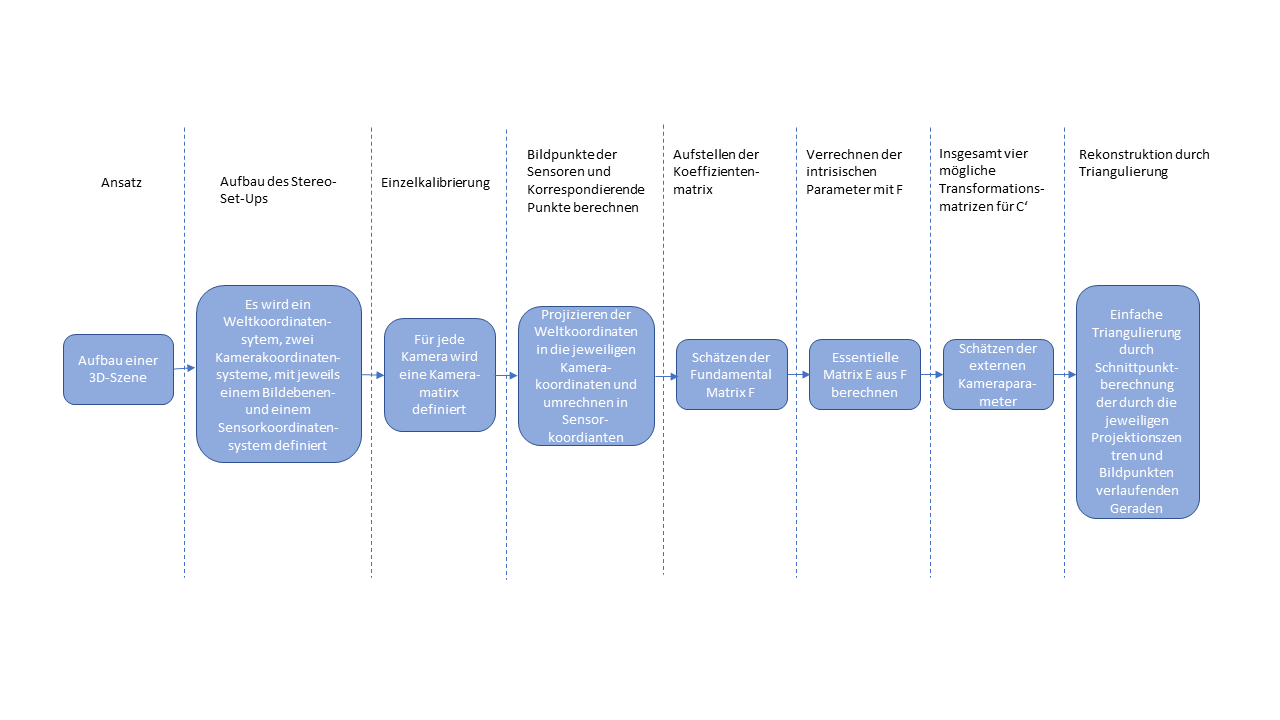
\includegraphics[width=1.\linewidth]{images/ArbeitsProzessMinimal.png}
	\captionof{figure}{Arbeitsprozesse der Stereoanalyse bei Verwendung von eigens erstellten synthetischen Bilddaten}
	\label{fig:ArbeitsProzessMinimal}
\end{minipage}\\ \\


\begin{minipage}{\linewidth}
	\centering
	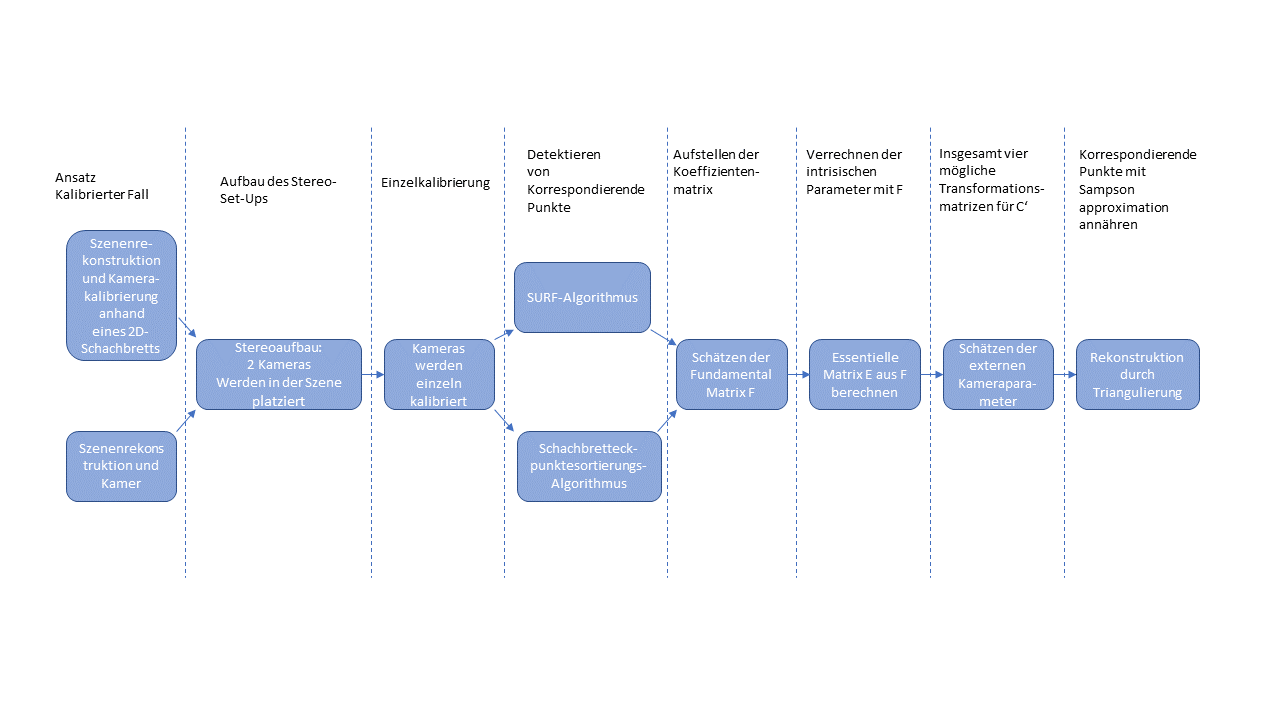
\includegraphics[width=1.\linewidth]{images/ArbeitsProzessReal.png}
	\captionof{figure}{Arbeitsprozesse der Stereoanalyse bei Verwendung von realen Bilddaten}
	\label{fig:ArbeitsProzessReal}
\end{minipage}\\ \\


Ein sehr wichtiger Aspekt dieses Ansatzes gerade im Bezug dann auch auf die Frage der Auswirkung von unterschiedlichen Kameraauflösungen auf die Szenerekonstruktion, ist die Epipolargeometrie. Sie beschreibt allem voran die zusammenhängende Geometrie zwischen den Bildpunkten zweier Bilder zueinander und deren geometrischen Zusammenhang zum 3D-Objektpunkt, was bei der Rekonstruktion der Szene besonders wichtig ist.\\


(Grafik Arbeitsprozess Unkalibrierter Fall nach Matlab) \\


In Abbildung ??? ist der Arbeitsprozess des unkalibrierten Falles aufgezeigt, so wie er beispielsweise in \textit{Matlab} implementiert ist. Der elementare Schritt mit dem sich beschäftigt wird ist die Rektifizierung der Bilder. Im Schritt der Rektifizierung wird die sogenannte geometrische Verzerrung zweier Bilder eliminiert, was genau das Bedeutet wird im Kapitel \nameref{sec:rectification} beschrieben. Die Rektifizierung beinhaltet vorallem mathematische Operationen auf den 2D-Bildebenen der aufgenommenen 2D-Bilder, weshalb im Zuge dessen die Funktion und Herleitung von Homographien im Kapitel \nameref{sec:homographien} aufgezeigt werden. Der Grund warum die Rektifizierung in den Vordergrund gerückt wird, ist, das es Beispielswesise genau in diesem Schritt in \textit{Matlab} zu einem Problem kommt, wenn mit Kameras unterschiedlicher Auflösung gearbeitet wird. Die Herkunft des Problems wird im Verlauf der Arbeit geklärt und ein Ansatz für Minimierung dessen, wenn man den unkalibrierten Fall verfolgen möchte, wird aufgezeigt. Zu finden ist dies im Kapitel \nameref{sec:rectification}.Die Kapitel sind wie folgt gegliedert. Kapitel 1 bis 5 umfassen die theoretischen Mathematischen Hintergründe, welche für das Verständnis der implementierten Kalibrierungs- und Rekonstruktionsalgorithmen vorhanden sein müssen. Kapitel 6 beinhaltet die einzelnen Schritte des in Abbildung \ref{fig:ArbeitsProzessMinimal} aufgezeigten Kalibrierungs- und Rekonstruktionsalgorithmus des Minimalbeispiels. Mit diesem Kapitel werden die zuvor beschriebenen mathematischen Werkzeuge zusammengefasst und in Bezug der Stereoskopischen Szenenrekonstruktion angewandt. Der Grund der implentierung dieses Minimalbeispiels war unter anderem der, dass somit Fehler, welche im Realbeispiel aufgetreten sind rekonstruiert und eine mögliche Lösung dieser ermittelt werden konnte. Kapitel 7 geht auf die Problematik der untschiedlichen Kamerauflösungen im Bezug auf die im Minimalbeispiel konstruierten Szene ein und führt auch noch auf, wie genau Auflösungen zustande kommen. Kapitel 8 und 9 transferieren dann den im Minimalbeispiel implementierten Algorithmus auf ein reales Beispiel mit einer echten Stereoskopischen Aufnahme. Die einzelnen Schritte aus Abbildung \ref{fig:ArbeitsProzessReal} werden hier ausführlichst besprochen. Das letzte Kapitel, Kapitel 10, bezieht sich auf einen Algorithmus welcher im Zuge des Realbeispiels enstanden ist. In Abbildung \nameref{fig:ArbeitsProzessReal} ist im Ansatz der Punkt Kalibrierung anhand eines 2D-Schachbretts aufgeführt. Der in Kapitel 10 beschriebene Algorithmus, kann die zuvor detektierten Punkte eines Schachbretts in eine Gitterstruktur sortieren, selbst wenn es zu starken Bildfehlern wie Verzeichnugen kommt und das Schachbrett auf Grund sender Lage auch noch projektiv verzerrt ist. Als Gitterstruktur sortiert bedeutet, dass die Punkte später wissen in welcher Zeile beziehungsweise Spalte sie sich im Gitternetz befinden und welches ihre Nachbarn sind. 

